
%(BEGIN_QUESTION)
% Copyright 2007, Tony R. Kuphaldt, released under the Creative Commons Attribution License (v 1.0)
% This means you may do almost anything with this work of mine, so long as you give me proper credit

A gas-fired heater is used to increase the temperature of a liquid feed, working to hold that temperature constant at the value specified by a local setpoint (LSP):

$$\includegraphics[width=15.5cm]{i01776x01.eps}$$

This simple control strategy may be adequate for most purposes, but there is room for improvement.  Consider, for instance, how the system will react if the temperature of the cold feed entering the heater suddenly increases.  Certainly, the temperature controller (TC) will take corrective action, but only after a rise in outlet temperature is sensed by the transmitter (TT).

One way to improve the system's response to changes is to add {\it feedforward} control.  Modify the control scheme to include a feedforward signal from a feed temperature transmitter, and explain how the modified system will be better than the system in place now.

\vskip 20pt \vbox{\hrule \hbox{\strut \vrule{} {\bf Suggestions for Socratic discussion} \vrule} \hrule}

\begin{itemize}
\item{} Perhaps the single most common mistake students make when planning a feedforward system is mis-placing the location of the {\it summing} function block, where the load signal adds to the feedback control signal.  Explain why the load signal should always be added to the feedback controller {\it output} signal, and never to the feedback controller {\it PV} signal.
\item{} What do you suppose the heating ``coils'' look like in real life?
\item{} For those who have already studied temperature measurement, what kind(s) of temperature-sensing elements do you think could be used in this application?
\item{} Are there any loads unaccounted for in the requested feedforward control strategy?  If so, see if you can modify this control strategy to account for them as well.
\end{itemize}

\underbar{file i01776}
%(END_QUESTION)





%(BEGIN_ANSWER)

The following P\&IDs show {\it incorrect} implementations of feedforward to this process.  All of these incorrect solutions are commonly seen among students first learning about feedforward control.

\vskip 20pt


\noindent
{\bf Incorrect solution \#1:} A mysterious third input on the temperature controller (TC) is being used here.  Although some loop controllers do provide an input for a feedforward transmitter's signal, to sketch this as a solution does not demonstrate understanding of the feedforward strategy.  What needs to be shown is a more explicit function-block strategy whereby it is clear to see what the feedforward signal actually does to achieve its ends.

$$\includegraphics[width=15.5cm]{i01776x06.eps}$$

\vskip 10pt

\filbreak



\noindent
{\bf Incorrect solution \#2:} Here we see the feedforward signal being summed with the process variable signal before it enters the controller.  The reason this won't work has to do with the purpose of the temperature controller (TC) -- to maintain the outgoing product temperature at some operator-determined setpoint (local setpoint, or LSP).  If that controller isn't able to directly and accurately sense the product temperature (because that temperature signal is being added to a different temperature signal) then there is no way the controller will ever be able to hold the product temperature to setpoint.  In other words, summing the two temperature signals together effectively ``lies'' to the controller such that it never sees the real process variable, and therefore can never hold the real process variable stable at setpoint because it's operating on false information.

$$\includegraphics[width=15.5cm]{i01776x04.eps}$$



\vskip 10pt

\filbreak


\noindent
{\bf Incorrect solution \#3:} In this solution the feedforward signal is being used as a remote setpoint (RSP) to the temperature controller (TC), much like you would expect to see in a {\it ratio} control system.  The trouble with this solution is again related to the purpose of the temperature controller -- to maintain the outgoing product temperature at some operator-determined setpoint.  Here there is no operator-determined setpoint at all, but rather a setpoint determined solely by the incoming feed temperature.  

$$\includegraphics[width=15.5cm]{i01776x05.eps}$$

Furthermore, it makes absolutely no sense at all to have the controller's setpoint made equal to the incoming feed temperature.  If we tried this strategy, the controller would maintain a closed-valve condition at all times, because the surest way to maintain the outgoing product temperature at a setpoint value equal to the incoming feed temperature is to not heat it up at all!



\vskip 10pt

\filbreak


\noindent
{\bf Incorrect solution \#4:} Similar to the last incorrect solution (\#3), this one attempts to use the feedforward signal as {\it part} of a remote setpoint value (RSP) to the temperature controller (TC), while still maintaining an operator-determined local setpoint (LSP).  Here we still have the same fundamental problem as before -- so long as the feedforward signal modifies either the controller's view of the process variable (the outgoing product temperature) or its setpoint, the controller will be unable to perform its most basic function, to maintain the outgoing product temperature at some operator-determined setpoint.

$$\includegraphics[width=15.5cm]{i01776x07.eps}$$




\vskip 10pt

\filbreak


\noindent
{\bf Incorrect solution \#5:} This solution comes closer than all the others with regard to conceptual correctness, but there is no way for it to be practically implemented.  One cannot simple merge two different control signals together (i.e. the temperature controller's output signal somehow joining together with the feedforward signal).  Whether these signals are physical (e.g. two 4-20 mA DC currents or two digital fieldbus messages), or virtual (e.g. binary values inside of a control system such as a DCS), we need some sort of algorithm to combine them together.  The two signals will simply not merge together in any sensible way on their own.

$$\includegraphics[width=15.5cm]{i01776x08.eps}$$


%(END_ANSWER)





%(BEGIN_NOTES)

The mathematical signs adjacent to the two summer inputs are critically important, especially the negative sign ($-$) next to the feedforward signal input.  These signs dictate the direction of action for each of the signal pathways (feedback and feedforward):

$$\includegraphics[width=15.5cm]{i01776x03.eps}$$

Truth be told, the sign at the summer's feedback input may be set either positive or negative, so long as the controller (TC) is configured to a corresponding action (direct vs. reverse) such that the entire feedback loop has a negative characteristic.  For example, we could use a noninverting summer input combined with a reverse-acting controller, or alternatively an inverting summer input with a direct-acting controller.

The feedforward summer input, however, {\it absolutely must} be inverting because this is the only way we have of defining the feedforward path's direction of action.  Since a hotter feed temperature needs to result in a more-closed fuel valve, the feedforward action must be reverse, and the summer's sign at that input is the only means we have of establishing a reverse action for the feedforward path.



\vfil \eject

\noindent
{\bf Summary Quiz:}

Identify the consequence of the temperature transmitter failing ``high'' (e.g. 20 mA) in this control system:

$$\includegraphics[width=15.5cm]{i01776x02.eps}$$

\begin{itemize}
\item{} The natural gas supply pressure will increase
\vskip 5pt 
\item{} The feed flow rate into the heater will decrease
\vskip 5pt 
\item{} The feed (liquid) pressure will increase
\vskip 5pt 
\item{} The liquid exiting the heater will become too hot 
\vskip 5pt 
\item{} The feed flow rate into the heater will increase 
\vskip 5pt 
\item{} The liquid exiting the heater will become too cold
\end{itemize}

%INDEX% Control, strategies: feedforward
%INDEX% Process: heater (fired) (generic)

%(END_NOTES)


